\begin{mainquestion}{diode_hogging}{Parallel Diodes}
We explore the case of two identical diodes placed in parallel as shown in the accompanying figure. Assume the diodes have $n = 1$. For each diode, a forward current of \qty{250}{\milli\ampere} results in a voltage of \qty{800}{\milli\volt} at \qty{300}{\kelvin}.

\begin{center}
    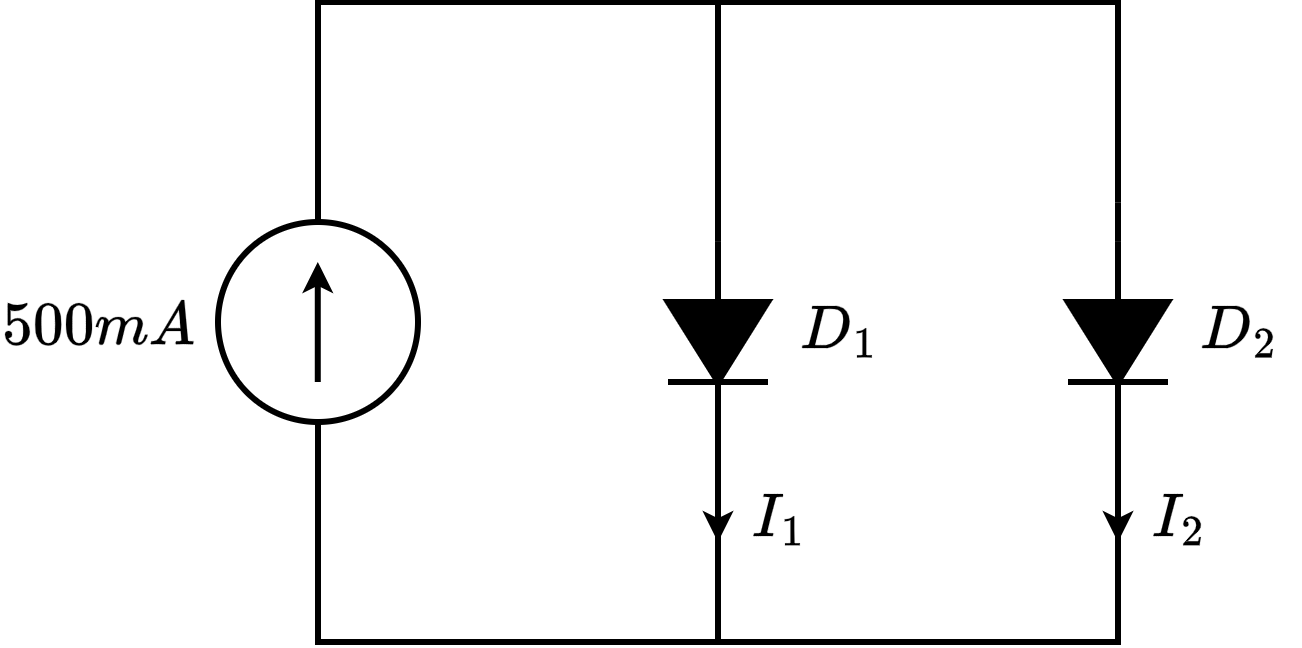
\includegraphics[width=0.5\textwidth]{questionbank/diodes/diode_hogging/v1/diode_schematic.png}
\end{center}

% =========================================================
\begin{partquestion}{current}
{If both diodes are at 300 K, what are the values of $I_1$ and $I_2$?}

\begin{answer}
Using KCL, $I_1 + I_2 = \qty{500}{\milli\ampere}$. Since the diodes are identical, by symmetry we expect $I_1 = I_2 = \qty{250}{\milli\ampere}$.
\end{answer}
\end{partquestion}

% =========================================================
\begin{partquestion}{currenthot}
{If diode 1 is at 300 K and diode 2 is at 310 K, find $I_1$ and $I_2$ using the rule of thumb that $I_S$ doubles every 5 K increase in temperature.}

\begin{answer}
We first determine $I_S$ at 300 K by plugging in known values of operation:
\[
I_S
=
I \exp\!\left(-\frac{qV_D}{nkT}\right)
=
\left(\qty{250}{\milli\ampere}\right)
\exp\!\left(-\frac{1.6\times10^{-19}\cdot0.800}{1\cdot1.38\times10^{-23}\cdot300}\right)
=
9.34\times10^{-15}\,\mathrm{A}
\]

Now we can find the diode currents:
\[
\qty{0.5}{\ampere}
=
I_1 + I_2
=
I_S \exp\!\left(38.65 V_D\right)
+
4 I_S \exp\!\left(37.40 V_D\right)
\]

Note the factor of 4 in the second term arises because when temperature increases by 10 K, $I_S$ quadruples. This is a transcendental equation that can be solved numerically using MATLAB, Newton’s method, graphically, or trial and error, resulting in $V_D = \qty{0.79436}{\volt}$.

It follows using
\[
I \approx I_S \exp\!\left(\frac{V_D}{nV_T}\right)
\]
that $I_1 = \qty{0.201}{\ampere}$ and $I_2 = \qty{0.299}{\ampere}$.
\end{answer}
\end{partquestion}

% =========================================================
\begin{partquestion}{heat}
{Based on your result from (\cref{prob:diode_hogging:currenthot}), which diode will heat up, and which will cool down?}

\begin{answer}
Diode 2, with an increase in current (from \qty{0.250}{\ampere} to \qty{0.299}{\ampere}), dissipates more power and therefore tends to heat further. Diode 1, with a decrease in current (from \qty{0.250}{\ampere} to \qty{0.201}{\ampere}), dissipates less power and therefore tends back toward its ambient temperature.
\end{answer}
\end{partquestion}

% =========================================================
\begin{partquestion}{hogging}
{What will happen to the diodes as their temperatures change? Describe the potential problem.}

\begin{answer}
As diode 2 continues to heat up, we know its current will continue to increase as well—a bit of undesired positive feedback. Over a short period of time, this can lead to “current hogging” and cause diode 2 to conduct nearly all of the current, while diode 1 sits relatively idle. Situations like this are undesirable because it is often easy to exceed the rated specifications and cause damage to a device if it is carrying more current than intended.
\end{answer}
\end{partquestion}

% =========================================================
\begin{partquestion}{solver}
{One possible mitigation for the problem discussed in (\cref{prob:diode_hogging:hogging}) is the addition of a series resistor $R$ in series with each diode. Find an expression for $R$ in terms of the currents $I_1$ and $I_2$ and the voltages $V_{D1}$ and $V_{D2}$.}

\begin{center}
    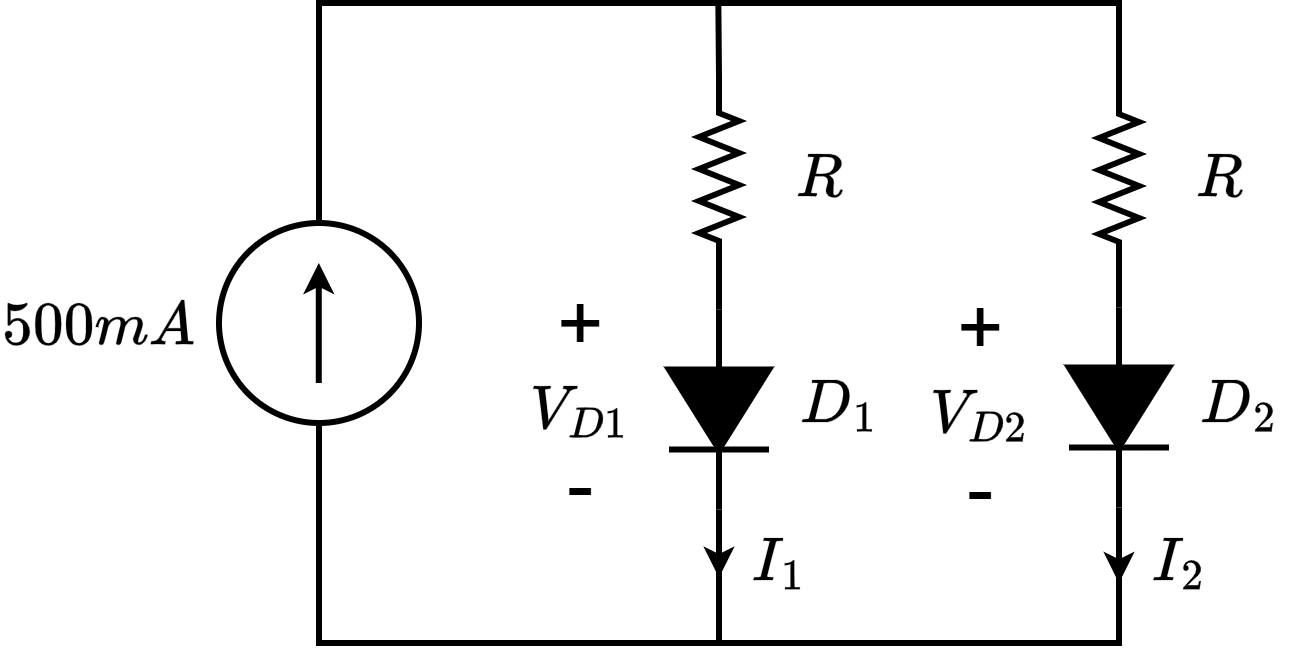
\includegraphics[width=0.5\textwidth]{questionbank/diodes/diode_hogging/v1/diode_rs_schematic.png}
\end{center}


\begin{answer}
Assuming a voltage $V$ across the current source, we can use Ohm’s law:
\[
I_1 = \frac{V - V_{D1}}{R}
\qquad
I_2 = \frac{V - V_{D2}}{R}
\]

Eliminating $V$ gives:
\[
I_1 R + V_{D1} = I_2 R + V_{D2}
\]

so
\[
R = \frac{V_{D2} - V_{D1}}{I_1 - I_2}.
\]
\end{answer}
\end{partquestion}

% =========================================================
\begin{partquestion}{findr}
{Find the value for $R$ that ensures the currents $I_1$ and $I_2$ are within 1\% of one another \textit{i.e.,} $I_{\mathrm{min}} \geq 0.99I_{\mathrm{max}}$, assuming the temperatures remain as they were in part (b).}

\begin{answer}
We have $I = I_1 + I_2$ and the constraint $I_1 \ge 0.99 I_2$. This implies $I_2 \le \frac{I}{1.99}$, giving $I_2 \le \qty{0.2513}{\ampere}$ and thus $I_1 \ge \qty{0.2487}{\ampere}$.

At equality:
\[
V_{D1} = \frac{nkT_1}{q}\ln\!\frac{I_1}{I_S}
\qquad
V_{D2} = \frac{nkT_2}{q}\ln\!\frac{I_2}{4I_S}
\]

where $T_1 = \qty{300}{\kelvin}$ and $T_2 = \qty{310}{\kelvin}$.

This gives $V_{D1} = \qty{0.7999}{\volt}$ and $V_{D2} = \qty{0.7897}{\volt}$. Then
\[
R = \frac{V_{D2} - V_{D1}}{I_1 - I_2}
=
\frac{0.7897 - 0.7999}{0.2487 - 0.2513}
=
\qty{3.92}{\ohm}.
\]

Anything that rounds to \qty{4}{\ohm} is acceptable.
\end{answer}
\end{partquestion}

% =========================================================
\begin{partquestion}{voltage}
{Calculate the voltage across the current source.}

\begin{answer}
Using $I_1 = \frac{V - V_{D1}}{R}$:
\[
V = I_1 R + V_{D1}
= (0.2487)(3.92) + 0.7999
= \qty{1.77}{\volt}.
\]

(We could have used the equivalent expression with $I_2$ and obtained the same result.)
\end{answer}
\end{partquestion}

% =========================================================
\begin{partquestion}{power}
{What is the ratio of the dissipated power in the two resistors to that of the remaining dissipated power?}

\begin{answer}
The total dissipated power is equal to the total supplied power
\[
VI = (1.77)(0.5) = \qty{0.885}{\watt}.
\]
The total power dissipated in the resistors (about 55\%) is
\[
I_A^2 R + I_B^2 R
=
(0.2487)^2(3.92) + (0.2513)^2(3.92)
=
\qty{0.490}{\watt}.
\]
and the remaining dissipated power must be 
\[
0.885 - 0.490 = \qty{0.395}{\watt}.
\]
all of which are consumed by the two diodes. The desired ratio is:
\[
\frac{0.490}{0.395} \approx 1.24.
\]
\end{answer}
\end{partquestion}

\end{mainquestion}